
Following from Lemma \ref{lem:transferdomination}, the current analysis studies the dual arm costs in the randomized unit tabletop setting, with $c_t$ as the cost measure per unit distance. 
For the $2$-arm setting, assume for simplicity that each arm's volume is represented as a disc of some radius 
$r$. For obtaining a $2$-arm solution, we partition the $n$ objects randomly 
into two piles of $\frac{n}{2}$ objects each; then obtain two initial solutions 
similar to the single arm case. It is expected (Eq.~\ref{eq:single-cost-simple}) that these two halves 
should add up to approximately $(c_{pd} + 0.52c_t)n$. 


From the initial $2$-arm solution, we construct an {\em asynchronous} $2$-arm 
solution that is collision-free. Assume that pickups 
and drop-offs can be achieved without collisions between the two arms, which 
can be achieved with properly designed end-effectors. The main overhead 
is then the potential collision between the two (disc) arms during transfer 
and move operations. Because there are $\frac{n}{2}$ objects for each arm to work 
with, an arm may travel a path formed by $n + 1$ straight line 
segments. Therefore, there are up to $(n + 1)^2$ intersections between the 
two end-effector trajectories where potential collision may happen. However,
because for the transfers and transits associated with one pair of objects (one 
for each arm) can have at most four intersections, there are at most 
$2n$ potential collisions to handle. For each intersection, let one 
arm wait while letting the other circling around it, which incurs a cost that is bounded by $2\pi \cdot
r \cdot c_t$. 


Adding up all the potential extra cost,  
% that a $2$-arm solution has 
a cumulative cost is obtained as 
% \begin{align}\label{eq:dual-cost-distance} 
% C_{dual} = C_{single} + 2n(2\pi rc_t) \approx (c_{pd} + 0.52c_t + 4\pi rc_t)n.
% \end{align}

{\centerline
{
$C_{\rm dual} = C_{\rm single} + 2n(2\pi rc_t) \approx (c_{pd} + 0.52c_t + 4\pi rc_t)n\;.$
}
}

\noindent For small $r$, $C_{\rm dual}$ is almost the same as $C_{\rm single}$ 
$c_t$ is a distance (e.g., energy) cost. Upon considering the maximum of the two arc lengths or makespan (Eq.~\ref{eq:cost_function}),
the $2$-arm cost becomes $C_{\rm dual}^t \approx (c_{pd} + 0.52c_t)\frac{n}{2} + 4n\pi rc_t$.
% \vspace{-0.1in}
% \begin{equation}\label{eq:dual-cost-time}
% C_{dual}^t \approx (c_{pd} + 0.52c_t)\frac{n}{2} + 4n\pi rc_t
% \vspace{-0.1in}
% \end{equation}
% {\centerline
% {
% $C_{dual}^t \approx (c_{pd} + 0.52c_t)\frac{n}{2} + 4n\pi rc_t$
% }
% }
The cost ratio is
\vspace{-0.1in}
\begin{equation}\label{eq:makespan-ratio}
\frac{C_{\rm dual}^t}{C_{\rm single}} \approx 
\frac{(c_{pd} + 0.52c_t)\frac{n}{2} + 4n\pi rc_t}{(c_{pd} + 0.52c_t)n}
= \frac{1}{2} + \frac{4\pi rc_t}{c_{pd} + 0.52c_t}\;.
% \vspace{-0.1in}
\end{equation}

\commentdel{
 \begin{wrapfigure}{r}{1.4in}
  \vspace{-.45in}
	\centering
    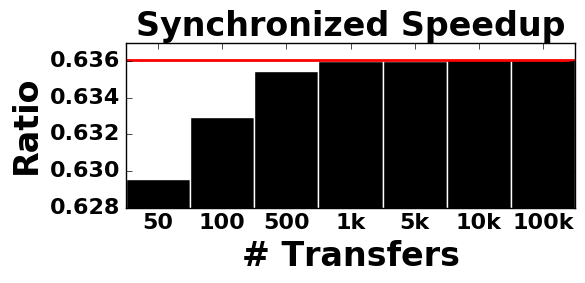
\includegraphics[width=1.4in]{figures/monte_carlo}
    \vspace{-.4in}
	\caption{Empirical cost ratio versus the estimate}
  	\label{fig:bounds}
    \vspace{-.4in}
\end{wrapfigure}
}

When $r$ is small or when $\frac{c_t}{c_{pd}}$ is small, the $2$-arm 
solution is roughly half as costly as the single arm solution. On 
the other hand, in this model a $2$-arm solution does not do better than $\frac{1}{2}$ of 
the single arm 
solution. This argument can be extended to $k$-arms as well.
\vspace{-0.08in}
\commentadd{
\begin{theorem}
For rearranging objects with non-overlapping starts and goals that are
uniformly distributed in a unit square,  a $2$-arm solution can have an 
asymptotic improvement of $\frac{1}{2}$ over the single arm solution. 
\label{thm:karm}
\end{theorem}
}
The synchronization assumption changes the expected cost of the solution. The random partitioning of the $n$ objects into two sets of $\frac{n}{2}$ object with a random ordering of the objects yields $\frac{n}{2}$ pairs of objects transfers, which dominate the total cost for large $n$. The cost~(Eq.~\ref{eq:cost_function}) of $\frac{n}{2}$ synchronized transfers ($\coma_i$) includes $\frac{n}{2}c_{pd}$ and $C^{\rm sync}_{sg} \approx (\mathtt{E}(max(l_1,l_2))c_t)\frac{n}{2}$, where $\mathtt{E}(max(l_1,l_2))$ is the expected measure of the max of lengths $l_1$,$l_2$ of two randomly paired transfers. Using the \textit{pdf}\cite{ghosh1951random} of lengths of random lines in an unit square and integrating over the setup, results in the value of $\mathtt{E}(max(l_1,l_2))$ to be $0.66$. 
% (Section \ref{sec:appendix}). 
This means $C_{\rm dual}^{\rm sync} \approx (c_{pd} + 0.66c_t)\frac{n}{2} + 4n\pi rc_t$.
% \vspace{-0.1in}
% \begin{equation}\label{eq:synchronized-cost}
% C_{dual}^{sync} \approx (c_{pd} + 0.66c_t)\frac{n}{2} + 4n\pi rc_t
% \vspace{-0.1in}
% \end{equation}
% {\centerline
% {
% $C_{dual}^{sync} \approx (c_{pd} + 0.66c_t)\frac{n}{2} + 4n\pi rc_t$
% }
% }
The synchronized cost ratio is
\vspace{-0.1in}
\begin{equation}\label{eq:synchronized-ratio}
\frac{C_{\rm dual}^{\rm sync}}{C_{\rm single}} \approx 
\frac{(c_{pd} + 0.66c_t)\frac{n}{2} + 4n\pi rc_t}{(c_{pd} + 0.52c_t)n}
= \frac{1}{2} + \frac{ (0.07 + 4\pi r)c_t}{c_{pd} + 0.52c_t}\;.
\vspace{-0.1in}
\end{equation}

When $\frac{c_t}{c_{pd}}$ is small, even the synchronized $2$-arm solution provides an improvement of $\frac{1}{2}$. For the case when both $r$ and $c_{pd}$ are small, we observe that the ratio approaches $0.636$. 
\commentdel{Fig \ref{fig:bounds} confirms empirically that in randomized trials on an unit square, the ratio of $\frac{C_{dual}^{sync}}{C_{single}}$ when $c_{pd}=0,r=0$, converges to the calculated estimate (red line).}
\vspace{-0.08in}
\begin{theorem}
For rearranging objects with non-overlapping starts and goals that are 
uniformly distributed in a unit square,  a randomized $2$-arm synchronized solution can have an 
asymptotic improvement of $\frac{1}{2}$ over the single arm solution if $\frac{c_t}{c_{pd}}$ is small, and a improvement $\approx 0.64$ when both $c_{pd}$ and $r$ are small. 
\end{theorem}

\commentadd{
\noindent \textbf{Note on bounds:} Even though the proposed simplified model does not apply immediately costs and collision volumes in general configuration spaces, experiments indicate that the speedups exist in these spaces as well.
}
% \rahul{this paragraph is phrased contradictorily. It makes sense if the first sentence is for asynchronous cases.}
% We note that the same can be said for a {\em synchronous} $2$-arm solution if
% when $c_t/c_{pd}$ is small. 
% Under the synchronization assumption, $C_{dual}^t$
% is no longer necessarily expected to be $\frac{C_{single}}{2}$ for large $n$. 
% Experiments in the next section indicate that improvements over single arm solutions in practical settings.

%\textcolor{red}{NOTE: We can also generate plots illustrating how the ratio 
%change as $n$, $r$, $c_{pd}:c_t$ changes. We may also further generalize the 
%$r$ based collision term to a more general collision term.}


%\begin{figure}[h]
%%  \begin{center}
%\centering
%    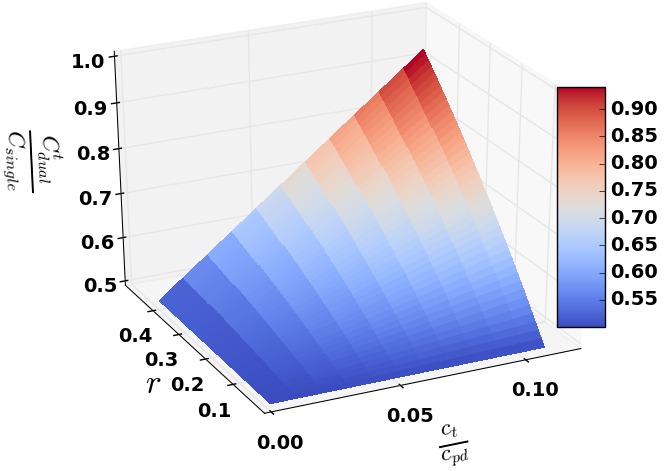
\includegraphics[width=2in]{figures/bounds}
%%  \end{center}
%  \caption{Bounds}
%  	\label{fig:bounds}
%\end{figure}


